\documentclass{beamer}
\usepackage[T1]{fontenc}
\usepackage[utf8]{inputenc}
\usepackage[french]{babel}
\usepackage{geometry}
\usepackage{graphicx}
\usepackage{wrapfig}
\usepackage{indentfirst}
\usepackage{tikz}
\usepackage{igo}
\usepackage{amsfonts}

\graphicspath{{/home/pgi/TIPE/content/Rapport/image/}}
\usetikzlibrary{trees}

% Title
\title{Morpion}
\author{Peng-Wei Chen, MP, \oldstylenums{2017}-\oldstylenums{2018}}
\date{}

\begin{document}
\tikzstyle{point}=[circle,draw,thin,fill=white]

\begin{frame}
    \titlepage
\end{frame}

\begin{frame}
    \frametitle{Avant-propos}
    \begin{itemize}
        \item La règle:
Deux joueurs jouent sur une grille de taille $15 \times 15$ sur le papier. Chacun prend un symbole et on dessine au tour par tour son symbole sur la grille. Le but est d'aligner 5 symboles verticalement, horizontalement ou en diagonale pour gagner.
%%fakesubsection
        \pause
        \item (m, n, k)-jeu
        \pause
        \item La stratégie gagnante a été trouvée.
        \item La borne inférieure de la taille de la grille dans laquelle il y a une stratégie gagnante n'est pas encore déterminée.
    \end{itemize}
    
\end{frame}


\begin{frame}
    \frametitle{Méthode}
    \begin{itemize}
        \item On cherche tous les cas possibles.
            \begin{itemize}
                \item L'arbre de décision
                    %%graphe de l'arbre
                \item Complexité O(($m 'times n$)!)
                \item{Fonction de valuation}
                \item k $\le$ 7
            \end{itemize}
        \item On apparie les points de la grille. Si le deuxième joueur peut toujours prévenir la réussite du premier joueur en jouant le pairage, alors une telle stratégie n'existe pas.\\
            k > 7

    \end{itemize}
\end{frame}


\begin{frame}
    \frametitle{Exploitation - k $\le$ 5}
    \framesubtitle{Fonction naïve}
    On considère le nombre de symboles non séparés dans une ligne.
    \begin{itemize}
        \item note d'un point sur la grille
        \item i-vivant / i-mort / mort
            {Figure. \ref{fig:vivmort}}
On donne $3^{i}$ au cas de i-vivant et $3^{i-1}$ au celui de i-mort car i-mort est en effet le cas de (i$-$1)-vivant. En particulier, on donne $3^{k+1}$ au cas où le premier joueur est sûrement gagné, c'est-à-dire k-mort ou (k-1)-vivant. 
        \item L'effet de directions differentes
Par exemple (Figure. \ref{fig:directions}), si k $=$ 5, le cas 4-mort-4-mort est un cas gagnant 
    \end{itemize}
    La \og note \fg \ est la somme de ces valeurs selon les quatre directions. 
\end{frame}

\begin{frame}
    \frametitle{Exploitation - k $\le$ 5}
    \framesubtitle{Fonction naïve}
    Exemple: fig:note
au point A, on somme 81 ($3^{4}$, horizontale) et $3\times 3$ ($3^1$,verticale et les deux directions diagonales). La note au point A vaut 90.
\end{frame}

\begin{frame}
    \frametitle{Exploitation - k $\le$ 5}
    \framesubtitle{L'élagage alpha-beta}
    \ref{fig:besoin}
    L'arbre de décision
    L'algorithme de minimax
        Note = difference des notes de deux joueurs
\ref{fig:minimax}

%% Exemple?
Dans l'arbre de décision, on donne la note de la position si c'est une feuille. Lorsqu'on est dans un nœud du niveau max (resp. min), on compare les notes de ses fils et en choisit la plus grande (resp. petite). En pratique, on se donne une hauteur et on fait un parcours en profondeur.\par
\end{frame}


%alpha-beta
\begin{frame}
    \frametitle{Exploitation - k $\le$ 5}
    \framesubtitle{L'élagage alpha-beta}
    L'élagage alpha-beta
    \ref{fig:alpha-beta}
    coupure alpha: niveau max
    coupure beta: niveau min
On utilise la fonction améliorée pour chercher la stratégie gagnante du premier joueur.
\end{frame}



%% k >= 8
\begin{frame}
    \frametitle{Exploitation - k $\ge$ 8}
    Le premier joueur n'a pas de stratégie gagnante lorsque k~=~8
        k~=~9: 
            \mbox{(Figure. \ref{fig:m-n-9})}
\end{frame}

\begin{frame}
    \frametitle{Exploitation - k $\ge$ 8}
    \framesubtitle{Preuve du cas k~=~8}
    Sous-jeu \ref{fig:sous-jeu} 
\end{frame}

\begin{frame}
    \frametitle{Exploitation - k $\ge$ 8}
    \framesubtitle{Preuve du cas k~=~8}
    Règle du sous-jeu: trois façons pour gagner  fig:regle
\begin{itemize}
    \item Aligner trois symboles en diagonale.
    \item Aligner verticalement deux symboles.
    \item Aligner horizontalement quatre symboles.
\end{itemize}
    
\end{frame}

\begin{frame}
    \frametitle{Exploitation - k $\ge$ 8}
    \framesubtitle{Preuve du cas k~=~8}
On peut montrer que le premièr joueur ne peut jamais gagner ce sous-jeu. On divise la grille initialle en des grilles du sous-jeu (Figure. \ref{fig:m-n-8}). Ainsi, 
    
\end{frame}

\begin{frame}
    \frametitle{Conclusion}
On suppose que $m \le n$.
Dans le cas où $k \le 5$, une telle stratégie existe lorsque
\begin{itemize}
    \item k = 3\\
        $m \ge 3$, $n \ge 4$
    \item k = 4\\
        $m \ge 4$, $n \ge 5$
    \item k = 5
\end{itemize}
Dans le cas où $k \ge 8$, il n'existe pas une stratégie gagnante pour le premier joueur.
\end{frame}

\section{Annexe}

f% Figure: arbre de decision
\begin{figure}[h]
    \centering
    \gobansize{3}
    \black{b2}
    \copytogoban{2}
    \white{a3}
    \copytogoban{3}
    \clear{a3}
    \white{a2}
    \copytogoban{4}
    \cleargoban
    \black{a2}
    \copytogoban{5}
    \clear{a2}
    \black{a3}
    \copytogoban{6}
    \clear{a3}

\begin{tikzpicture}[level distance=2cm,
    level 1/.style={sibling distance=4cm},
level 2/.style={sibling distance=1.5cm}]
  \node {\showfullgoban}
  child {node {\usegoban{2} \showfullgoban}
      child {node {\usegoban{3} \showfullgoban}
      child {node {$\vdots$}}}
      child {node {\usegoban{4} \showfullgoban}
      child {node {$\vdots$}}}
    }
    child {node {\usegoban{5} \showfullgoban}
        child {node {$\vdots$}}
        child {node {$\vdots$}}
    }
    child {node {\usegoban{6} \showfullgoban}
        child {node {$\vdots$}}
        child {node {$\vdots$}}
    };
\end{tikzpicture}
    \caption{Arbre de décision (le cercle noir est le symbole du premier joueur)} \label{fig:arbre}
\end{figure}

\gobansize{10}
\cleargoban

%% Exemple: 3-vivant, 3-mort
\begin{figure}[h]
    \centering
        \black{d5,e5,f5}
        \shortstack{\showgoban\\3-vivant}
        \white{g5}
        \shortstack{\showgoban\\3-mort}
    \\
    \ \\
        \white{c5}
        \clear{e5}
        \gobansymbol{e5}{A}
        \shortstack{\showgoban\\La note au point A est nulle pour le noir.}
    \caption{3-vivant et 3-mort}
    \label{fig:vivmort}
\end{figure}

\cleargoban
%% Exemple: 2 directions
\begin{figure}[h]
    \centering
        \black{d5,e5,f5,g3,g4,g6}
        \white{c5,g7}
        \black[\igotriangle]{g5}
        \gobansymbol{h5,g2}{x}
        \shortstack{\showgoban}
    \caption{L'effet des directions différente}
    \label{fig:directions}
\end{figure}
\cleargoban

%% Exemple: note 
\begin{figure}[h]
    \centering
        \black{d5,e5,f5}
        \gobansymbol{g5}{A}
        \shortstack{\showgoban}
    \caption{Un exemple de la note}
    \label{fig:note}
\end{figure}

%% Exemple: Besoin de alpha-beta
\begin{figure}[h]
    \centering
    \cleargoban
    \gobansize{5}
    \black[1]{c3}
    \white[2]{b4}
    \shortstack{\showfullgoban\\1}
    \cleargoban
    \black{c3}
    \white{b4}
    \white[\igotriangle]{b2,c2,d3,d4}
    \shortstack{\showfullgoban\\2}
    \cleargoban
    \black{c3,d3}
    \white{b4}
    \white[\igotriangle]{b3}
    \shortstack{\showfullgoban\\3}
    \caption{Insuffisance de notre fonction naïve}
    \label{fig:besoin}
\end{figure}

%% Exemple: minimax
\begin{figure}[h]
    \centering
    \begin{tikzpicture}[level distance=2cm,
        level 1/.style={sibling distance=4cm},
        level 2/.style={sibling distance=4cm},
        level 3/.style={sibling distance=1.5cm}]
        \node[point] (n){\ }
            child {node (n0){27}
                child {node (n1){27}
                    child {node {4}}
                    child {node (n2){27}}
                    child {node {13}}
                }
                child {node (n3){29}
                    child {node {2}}
                    child {node {23}}
                    child {node (n4){29}}
                }
            }
            child {node[point] (n5){\ }
            child {node (n6){$\vdots$}}
        };
        \node[right of=n5,node distance=4cm] {max};
        \node[right of=n6,node distance=4cm] {min};
        \node[right of=n4,node distance=4.5cm] {max};
        \node[right of=n,node distance=6cm] {Origine};
        \draw[->,draw=red] (n2) -- (n1);
        \draw[->,draw=red] (n4) -- (n3);
        \draw[->,draw=red] (n1) -- (n0);;
    \end{tikzpicture}
    \caption{L'algorithme de minimax}
    \label{fig:minimax}
\end{figure}

\begin{figure}[h]
    \centering
    \begin{tikzpicture}
%%alpha
        \node[point] (n0){\ }
        child {node {81}}
        child {node[point] (n1){A}
            child {node (n2){105}}
            child {node (n3){41}}
        }
        ;
        \node[right of=n1,node distance=2cm] {max};
        \node[right of=n3,node distance=1.3cm] {min};
        \node[below of=n2,node distance=0.5cm] {Coupure alpha};
        \draw[-] (n3) to node{X} (n1);
        \draw[-] (n1) to node{X} (n0);
%%beta
        \node[point,right of=n0,node distance=7cm] (n){\ }
        child {node {40}}
        child {node[point] (n4){\ }
            child {node (n5){35}}
            child {node (n6){77}}
        }
        ;
        \node[right of=n4,node distance=2cm] {min};
        \node[right of=n6,node distance=1.3cm] {max};
        \node[below of=n5,node distance=0.5cm] {Coupure beta};
        \draw[-] (n6) to node{X} (n4);
        \draw[-] (n4) to node{X} (n);
    \end{tikzpicture}
    \caption{L'algorithme de l'élagage alphaa-beta}
    \label{fig:alpha-beta}
\end{figure}

%% m-n-9
\begin{figure}[h]
    \centering
    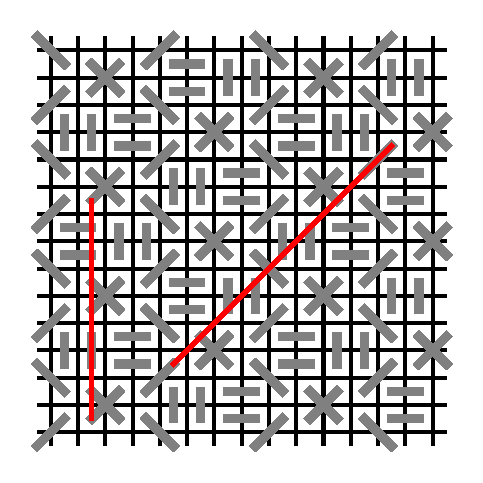
\includegraphics{m-n-9.eps}
    \caption{(m, n, 9)-jeu}
    \label{fig:m-n-9}
\end{figure}

%% sous-jeu
\begin{figure}[h]
    \centering
    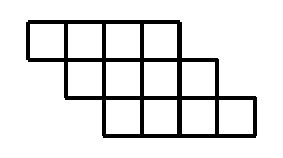
\includegraphics{m-n-8-little.eps}
    \caption{La grille du sous-jeu}
    \label{fig:sous-jeu}
\end{figure}

%% regle de sous-jeu
\begin{figure}[h]
    \centering
    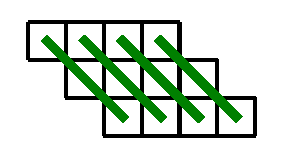
\includegraphics{8-rules1.eps}
    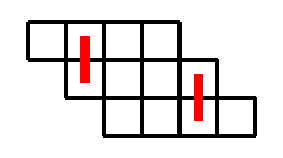
\includegraphics{8-rules2.eps}
    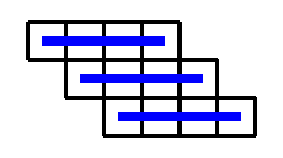
\includegraphics{8-rules3.eps}
    \caption{Les trois façons pour gagner le sous-jeu.}
    \label{fig:regle}
\end{figure}

%% m-n-8
\begin{figure}[h]
    \centering
    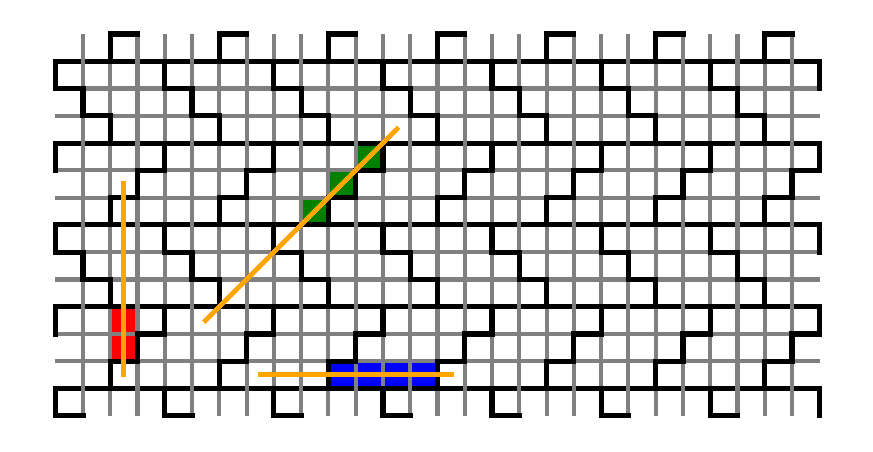
\includegraphics{8-sol.eps}
    \caption{(m, n, 8)-jeu:
    toutes les lignes de longueur 8 passent une des lignes gagantes du sous-jeu.}
    \label{fig:m-n-8}
\end{figure}
\end{document}
